\section{Simulation}\label{section:Simulation}
We now cover the simulation work that we have done in order to analyze the fairness of the game and the performance of the proposed practical strategies.

For the sake of clarity, in this section we are going to refer to a generic player 1 as P1 and to player 2 as P2 for simplicity.

In order to understand if there is an inherent advantage in going first or second, we run several simulations and compare the outcomes of the games under all the combinations of two strategies from the ones explained in section \ref{section: Strategies}. In particular, we consider two cases:
\begin{itemize}
	\item General case: whoever starts between P1 and P2 is decided by which player gets the card 2 in its hand.
	\item P1 always starts: player P1 always gets the hand containing the 2, thus playing first.
\end{itemize}
To achieve our objective, we first generate $n$ pairs of random hands, one for each player. Then for each pair of hands, we simulate the game on every possible combination of two strategies from Section \ref{section: Strategies}.
We make the simplifying assumption of players sticking to their selected strategy. Obviously, this abstracts us from the human-playing scenario; however, it is an abstraction without loss of generality, since our focus is in finding evidence of an intrinsic unfairness of the game that must remove itself of any human-like factors.

Specifically, the simulations have been run on Google Colab with default configuration\footnote{Intel(R) Xeon(R) CPU @ 2.20GHz, 13 GB of RAM}, for a total of $n = 10000$ simulations of random hands for all possible combinations of strategies. This number of runs has been chosen in order to guarantee both a high enough sample size and a feasible computational time.

\subsection{Outcome analysis} \label{subsection: Outcomes}

In this section we cover the analysis of the game outcomes (win, lose, tie), both under the fairness aspect and the performance of strategies.

\begin{figure}
	\centering
	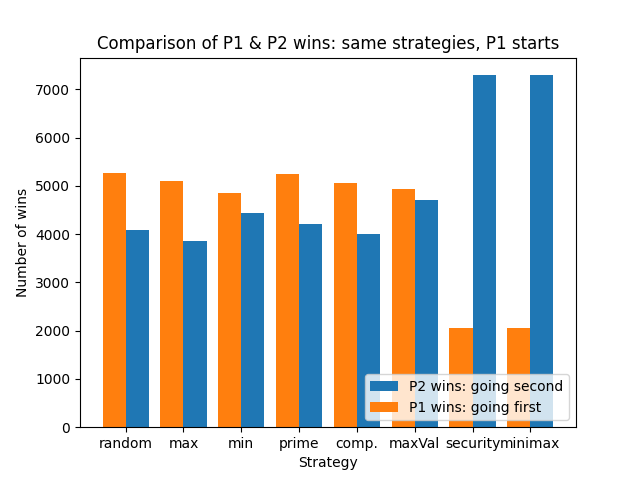
\includegraphics[width=1\linewidth]{img/histogram_p1vsp2_p1first.png}
	\caption{Number of wins of P2 vs P1 when P1 starts; both players play the same strategy.}
	\label{fig:hist_p1vsp2_p1first}
\end{figure}

\begin{figure}
	\centering
	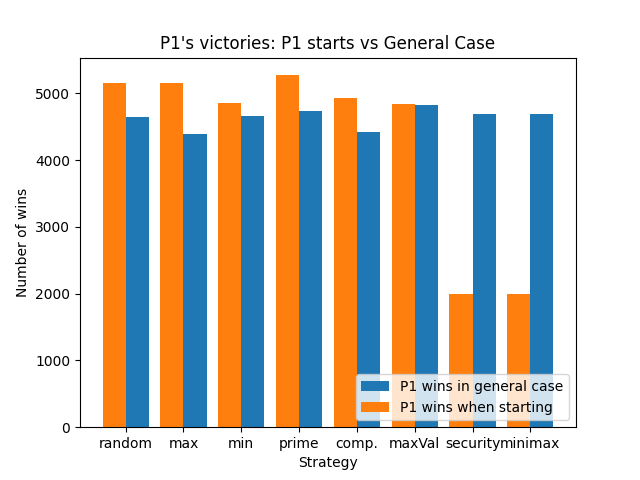
\includegraphics[width=1\linewidth]{img/histogram_p1wins_2cases.png}
	\caption{Number of wins of P1 when starting vs the general case; both players play the same strategy.}
	\label{fig:hist_p1wins_2cases}
\end{figure}

%\begin{figure}
%	\centering
%	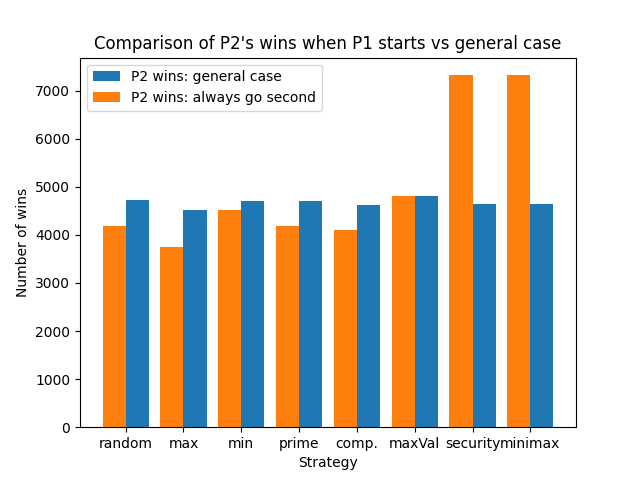
\includegraphics[width=1\linewidth]{img/histogram_p2wins_2cases.png}
%	\caption{Number of wins of P2 when P1 starts vs the general case; both players play the same strategy.}
%	\label{fig:hist_p2wins_2cases}
%\end{figure}

 Our analysis starts by considering Figures \ref{fig:hist_p1vsp2_p1first} and \ref{fig:hist_p1wins_2cases} where the two players play the same strategies.
 Those figures highlight the following points about the fairness of the game:
 \begin{itemize}
 	\item There is an advantage in going first for some strategies, i.e. random, max, min, prime, comp;
 	\item The situation is more or less balanced when playing the max\_value strategy;
 	\item There is a significant advantage in going second when both players play a either the security or minimax strategy;
 \end{itemize}
 A combined observation of these points is quite interesting: it seems that there is an advantage in going first when using stupid primitive strategies, but for more advanced ones the situation is flipped. An accurate analysis of this behaviour is quite difficult, given in particular the random nature of some of the strategies, however we propose an intuition to motivate it: a player using more advanced strategies and going second takes more opportunities to strategically form arithmetical operations with the cards visible on the table, considering also the potential opponent response, and thus achieve a greater number of points right from the first turns. This intuition is also supported by the more or less balanced behaviour of the max\_val pair, where each player tries to get the maximum partial payoff out of the current game state but without strategically looking ahead on the consequences of its action.

\begin{figure}
	\centering
	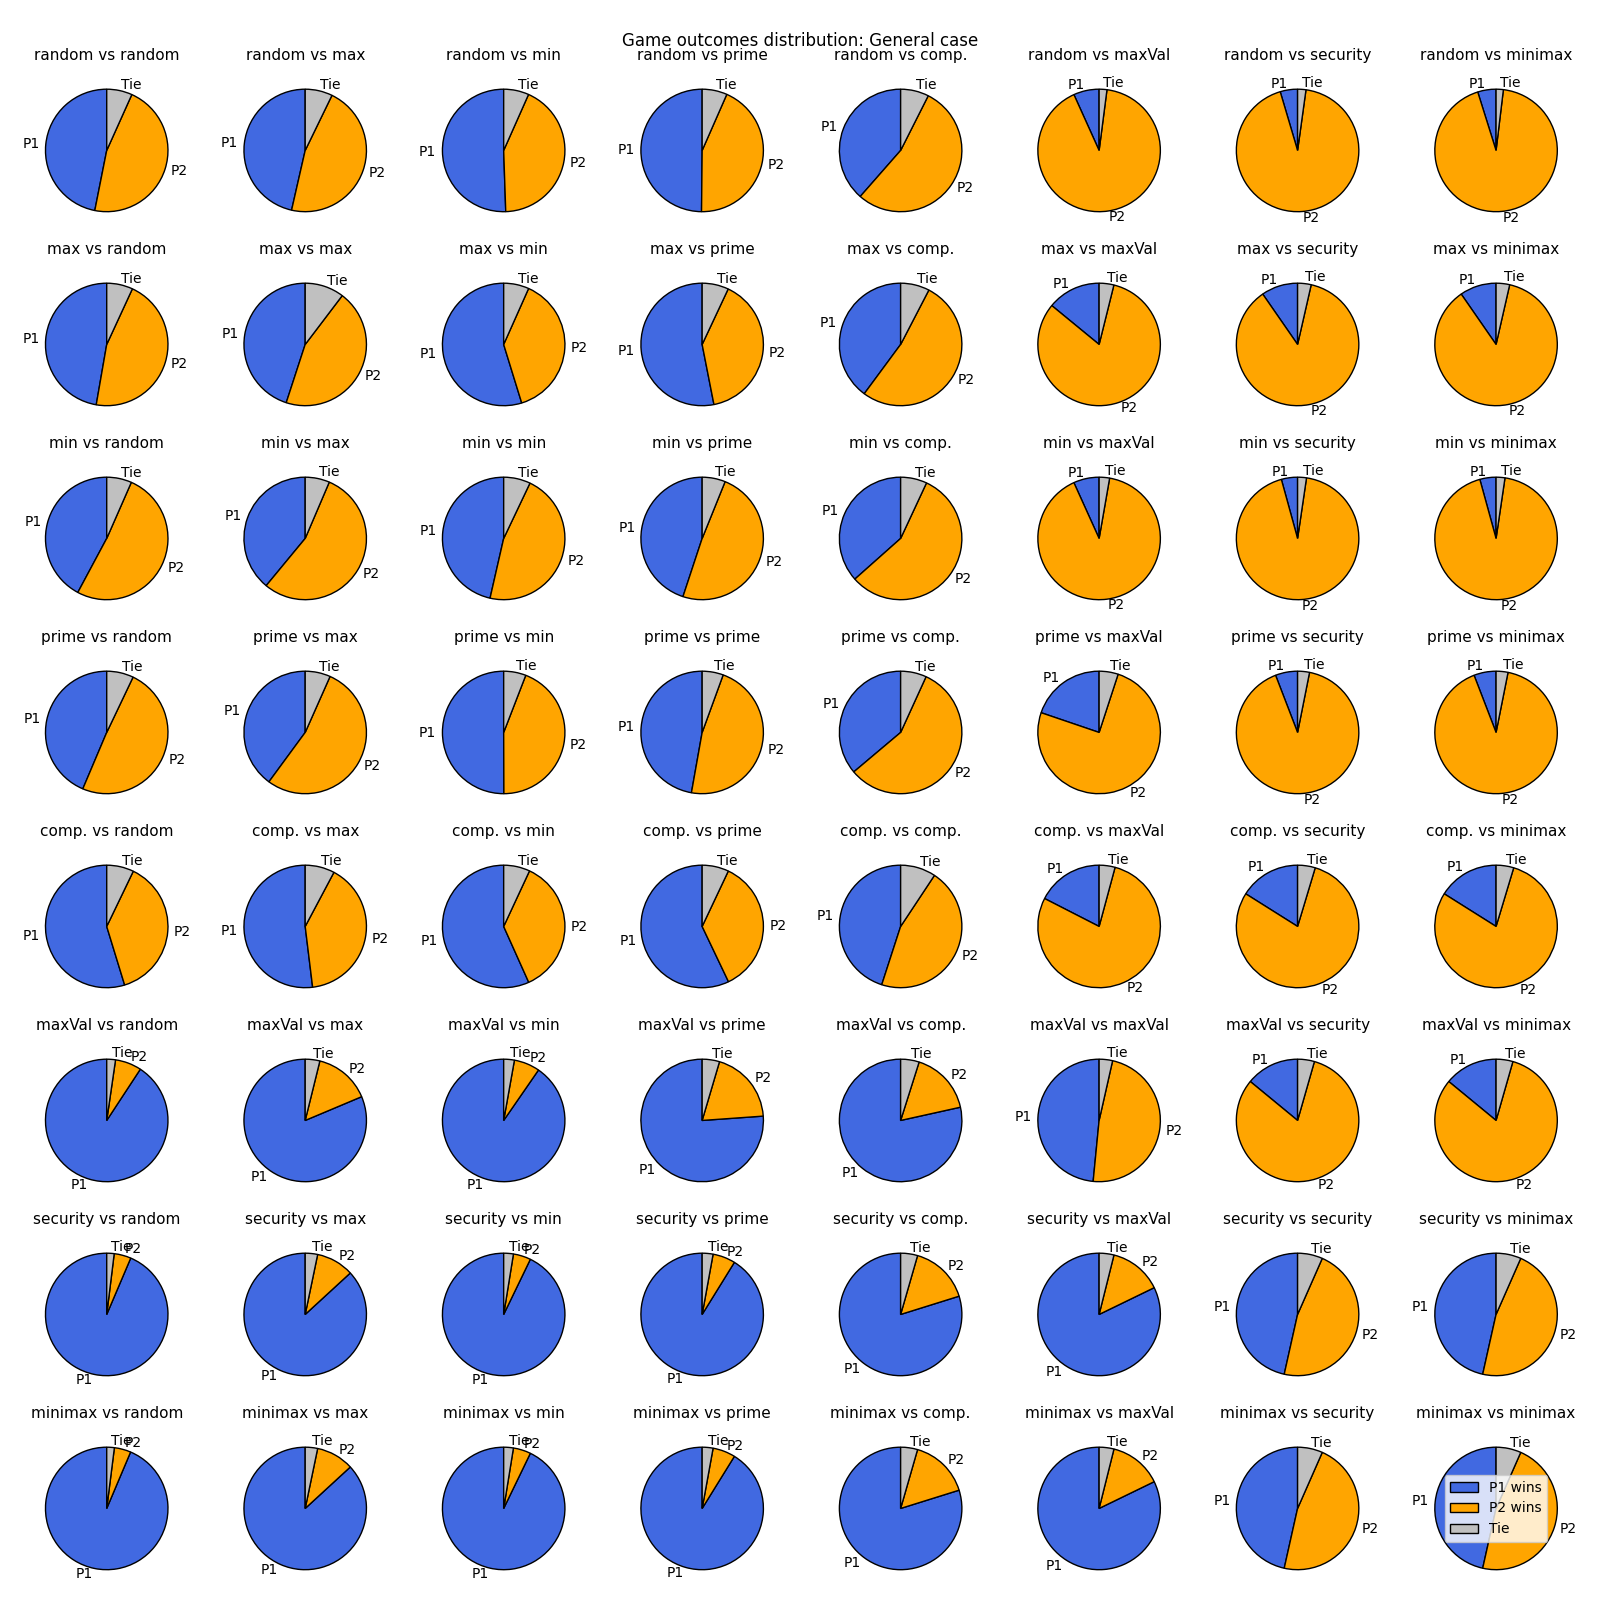
\includegraphics[width=1\linewidth]{img/outcomes_distribution_general.png}
	\caption{Outcomes distribution under all possible strategies combinations in the general case.}
	\label{fig:outcomes_distribution_general}
\end{figure}

\begin{figure}
	\centering
	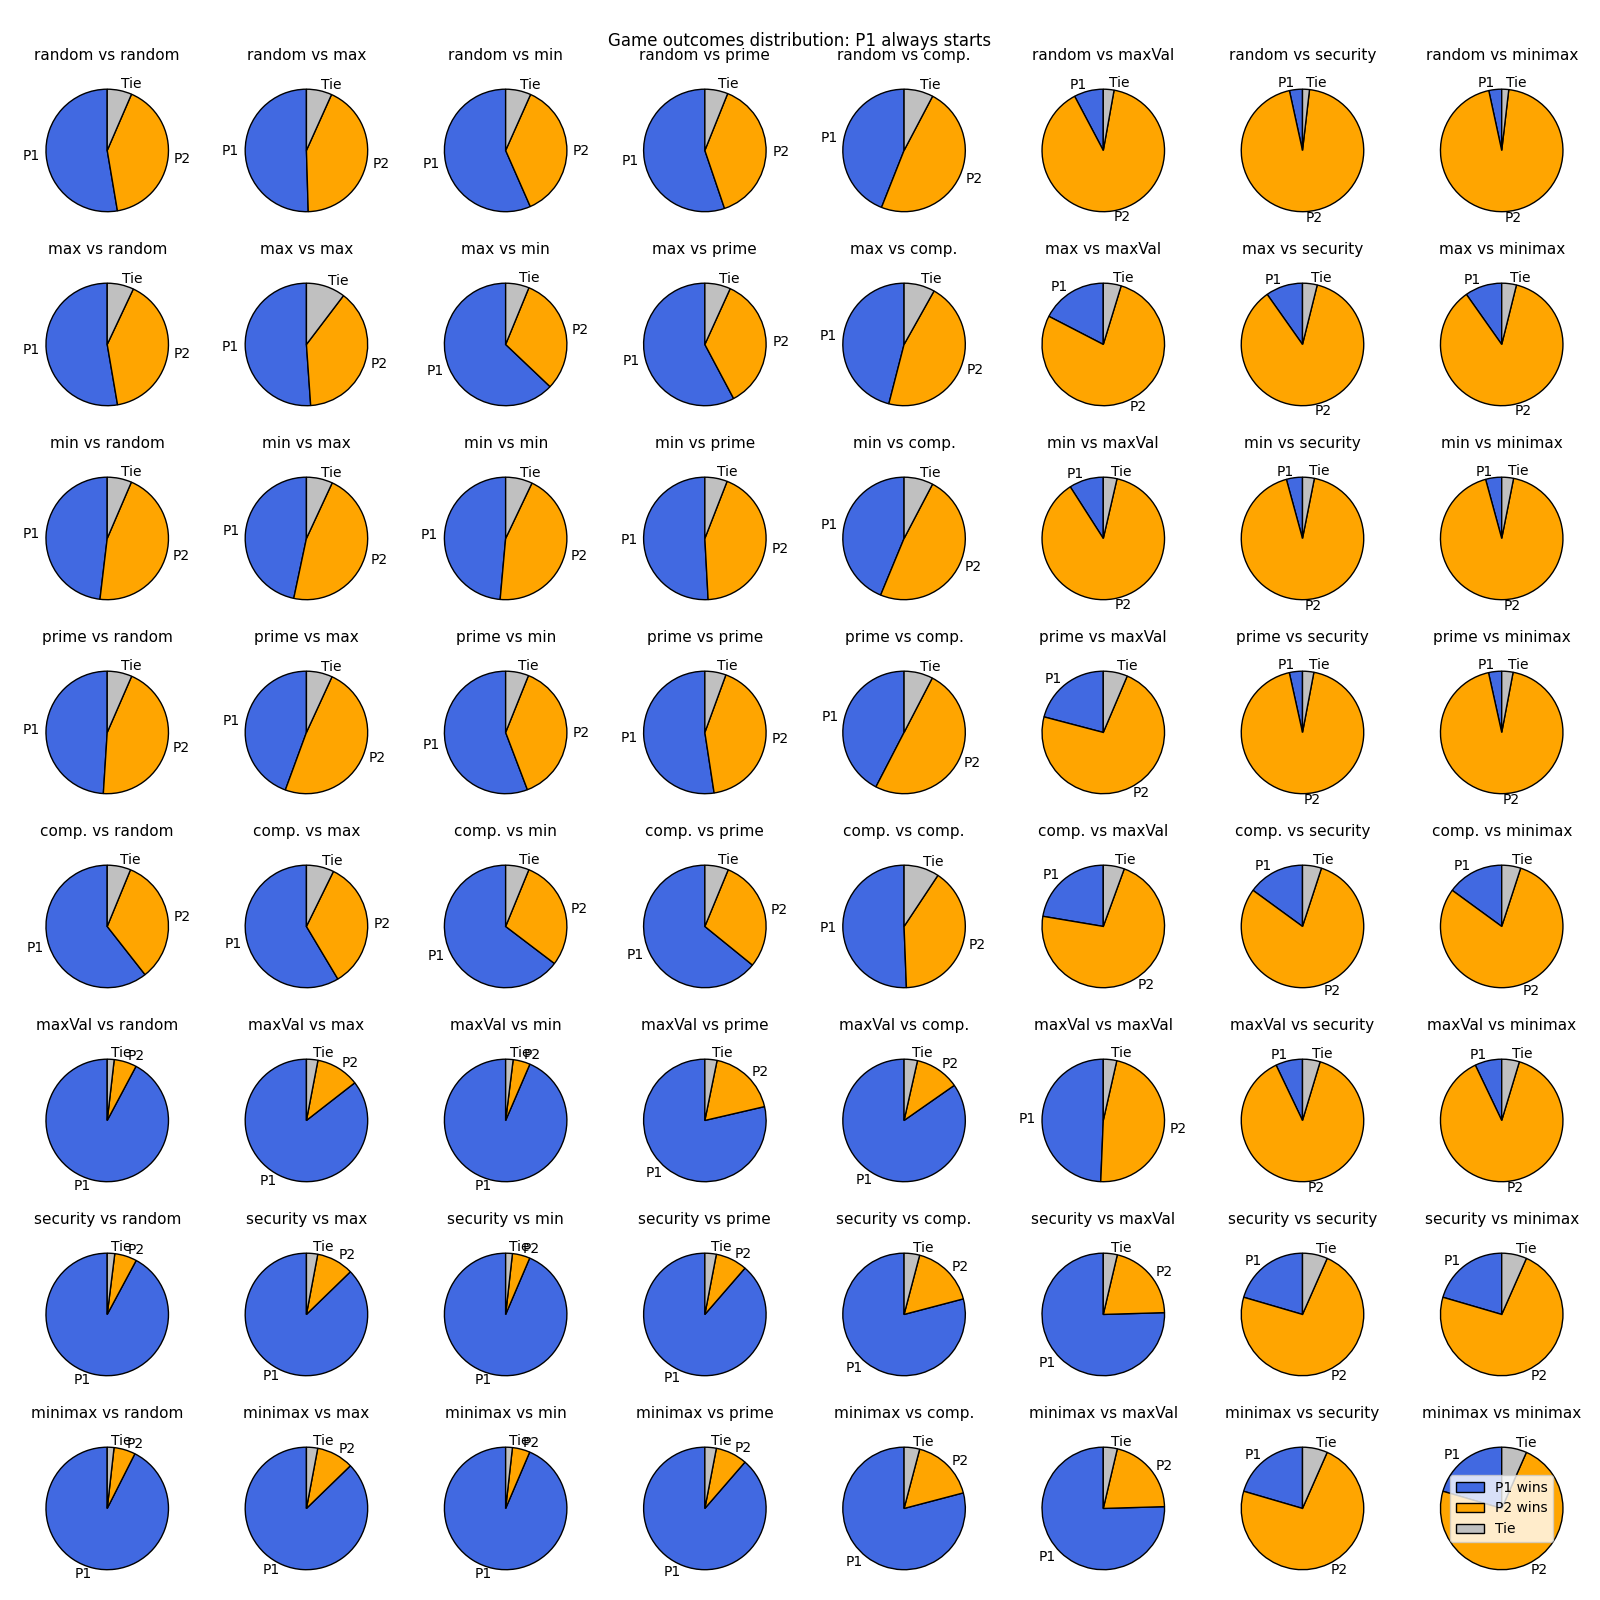
\includegraphics[width=1\linewidth]{img/outcomes_distribution_p1first.png}
	\caption{Outcomes distribution under all possible strategies combinations when P1 starts.}
	\label{fig:outcomes_distribution_p1first}
\end{figure}

Figures \ref{fig:outcomes_distribution_general} and \ref{fig:outcomes_distribution_p1first} strengthen those observations and expand on them, by allowing to see the distribution of wins for each player under all possible strategies combinations, in the general and P1-first cases respectively.
In particular, it is easy to see that there is an evident advantage in using zero-sum-like strategies in both cases. This was expected, since those two practical strategies are the ones that approximate more closely actual best-response strategies.
Additionally, we can see again the advantage in always going second when playing such strategies.

On the same note, also the max\_val	strategy performs quite well against the more primitive strategies, being based on the idea of "best play in a vacuum"; however, it gets outperformed by the zero-sum strategies, an expected result given their nature.

More importantly, those two figures allow us to discuss the fairness of the game on the whole: when considering the diagonals of the two figures (in other words players playing the same strategy), we clearly see that in the general case the situation is always more or less balanced, something that we do not see when we force P1 to go first. This allows us to conclude that the game is fair on the whole, but this fairness is more related to the randomized nature of whoever starts, i.e. whoever gets the 2 card, rather than the intrinsic characteristics of the game.

\begin{figure}
	\centering
	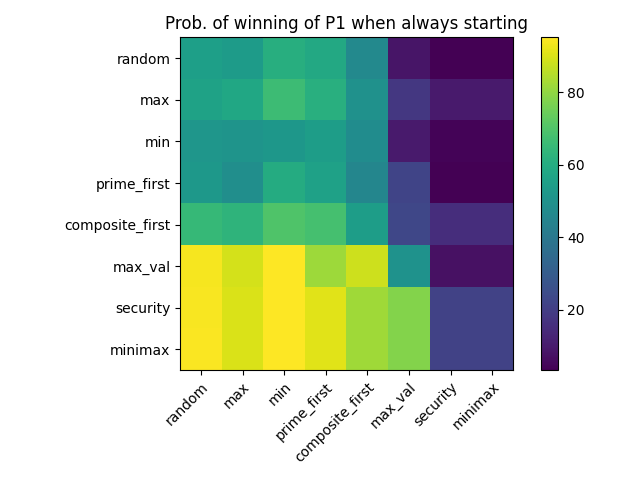
\includegraphics[width=1\linewidth]{img/prob_p1first.png}
	\caption{Heatmap of the probability of P1 winning when always going first.}
	\label{fig:prob_p1first}
\end{figure}

\begin{figure}
	\centering
	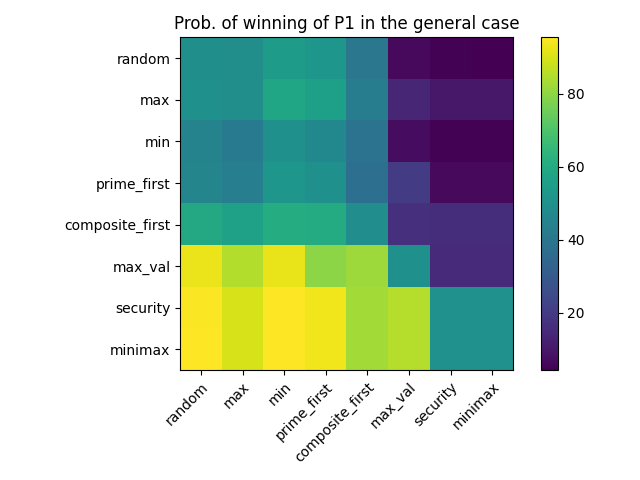
\includegraphics[width=1\linewidth]{img/prob_general.png}
	\caption{Heatmap of the probability of P1 winning in the general case.}
	\label{fig:prob_general}
\end{figure}

\begin{figure}
	\centering
	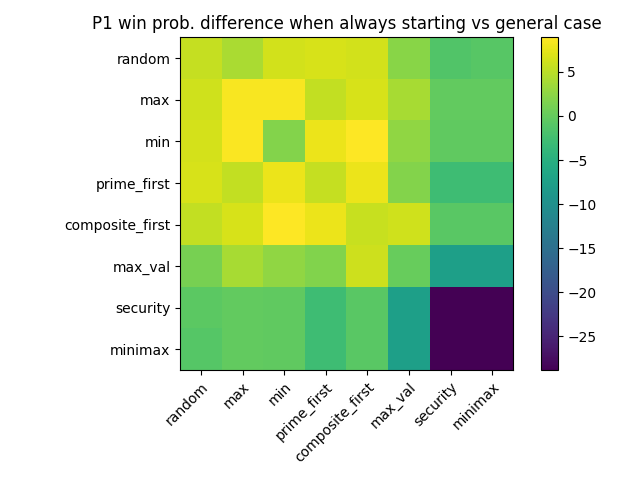
\includegraphics[width=1\linewidth]{img/prob_diff.png}
	\caption{Difference in probability of P1 winning when always going first vs in the general case.}
	\label{fig:prob_diff}
\end{figure}

In Figures \ref{fig:prob_general} and \ref{fig:prob_p1first} we show the probability of P1 winning under all the different strategy combinations as heat-maps for the two study cases.
The situation that we are presented with is quite similar to the one that we presented in Figures \ref{fig:outcomes_distribution_general} and \ref{fig:outcomes_distribution_p1first}, additionally highlighting the symmetrical situations across the diagonals.

However, the most interesting result is presented in Figure \ref{fig:prob_diff}, where the difference in victory probability of P1 between the P1-always-starts case and the general case is shown. The key takeaways are:
\begin{itemize}
	\item When considering simple primitive strategies, there is a slight advantage by always going first;
	\item When considering the more advanced strategies, there is a great difference in probability of victory between always starting and the general case, favouring going second;
\end{itemize}

To wrap up the outcomes analysis:
\begin{itemize}
	\item We have shown that more skilled players, i.e. players using advanced strategies, significantly outperform players using more simple strategies;
	\item Interestingly enough, we have seen that between low skilled players using primitive strategies the first one to move is favoured, however, the situation flips as soon as skilled players with advanced strategies come into play, favouring going second;
	\item Randomizing the hands, and thus whoever starts (general case), makes the game fair as a whole when considering players of "same skill level" (in other words, strategies of comparable complexity); however, this has more to do with the properties of randomization than the innate characteristics of the game.
\end{itemize}

At the end of the code, there is also a small part that uses an optimization method to find the binomial distribution that best fits the data in the two cases. The distributions found are very similar to the ones computed before.

\subsection{Scores analysis} \label{subsection:scores}

In our simulations, we have not only considered the outcomes of the simulated games but also the scores achieved by the players.
We then used these results in order to build box plots for each pair of strategies in the two cases that we have analysed, which can be seen in Figure \ref{fig:box_general} and \ref{fig:box_starts}. In all these plots, the first box shows the scores distribution for P1, while the second one of P2.

\begin{figure}
	\centering
	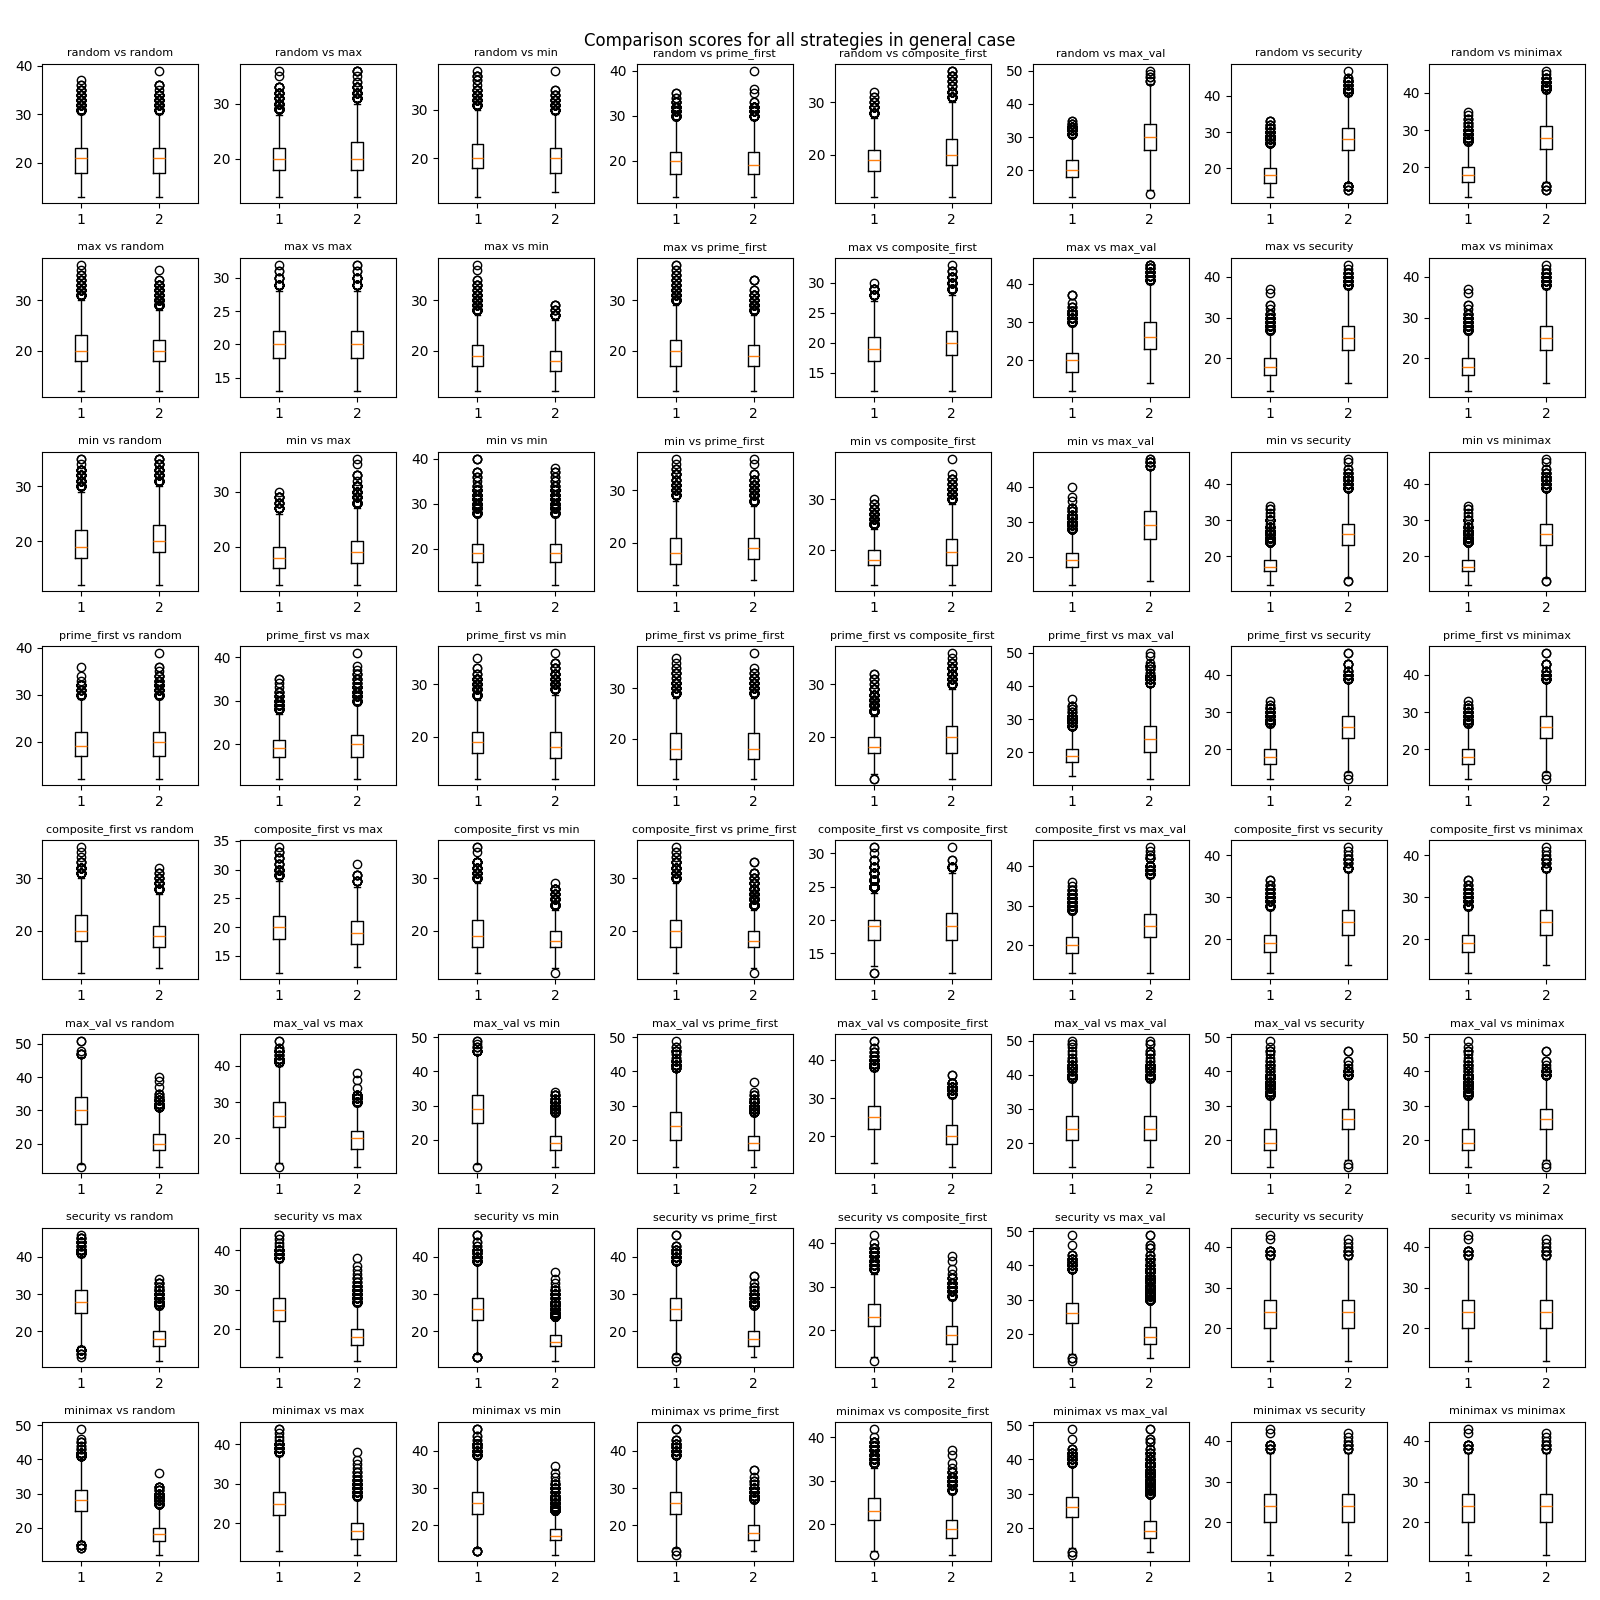
\includegraphics[width=1\linewidth]{img/scores_general.png}
	\caption{Plot that reports the box plots of the different score for each pair of strategies in the general case.}
	\label{fig:box_general}
\end{figure}

\begin{figure}
	\centering
	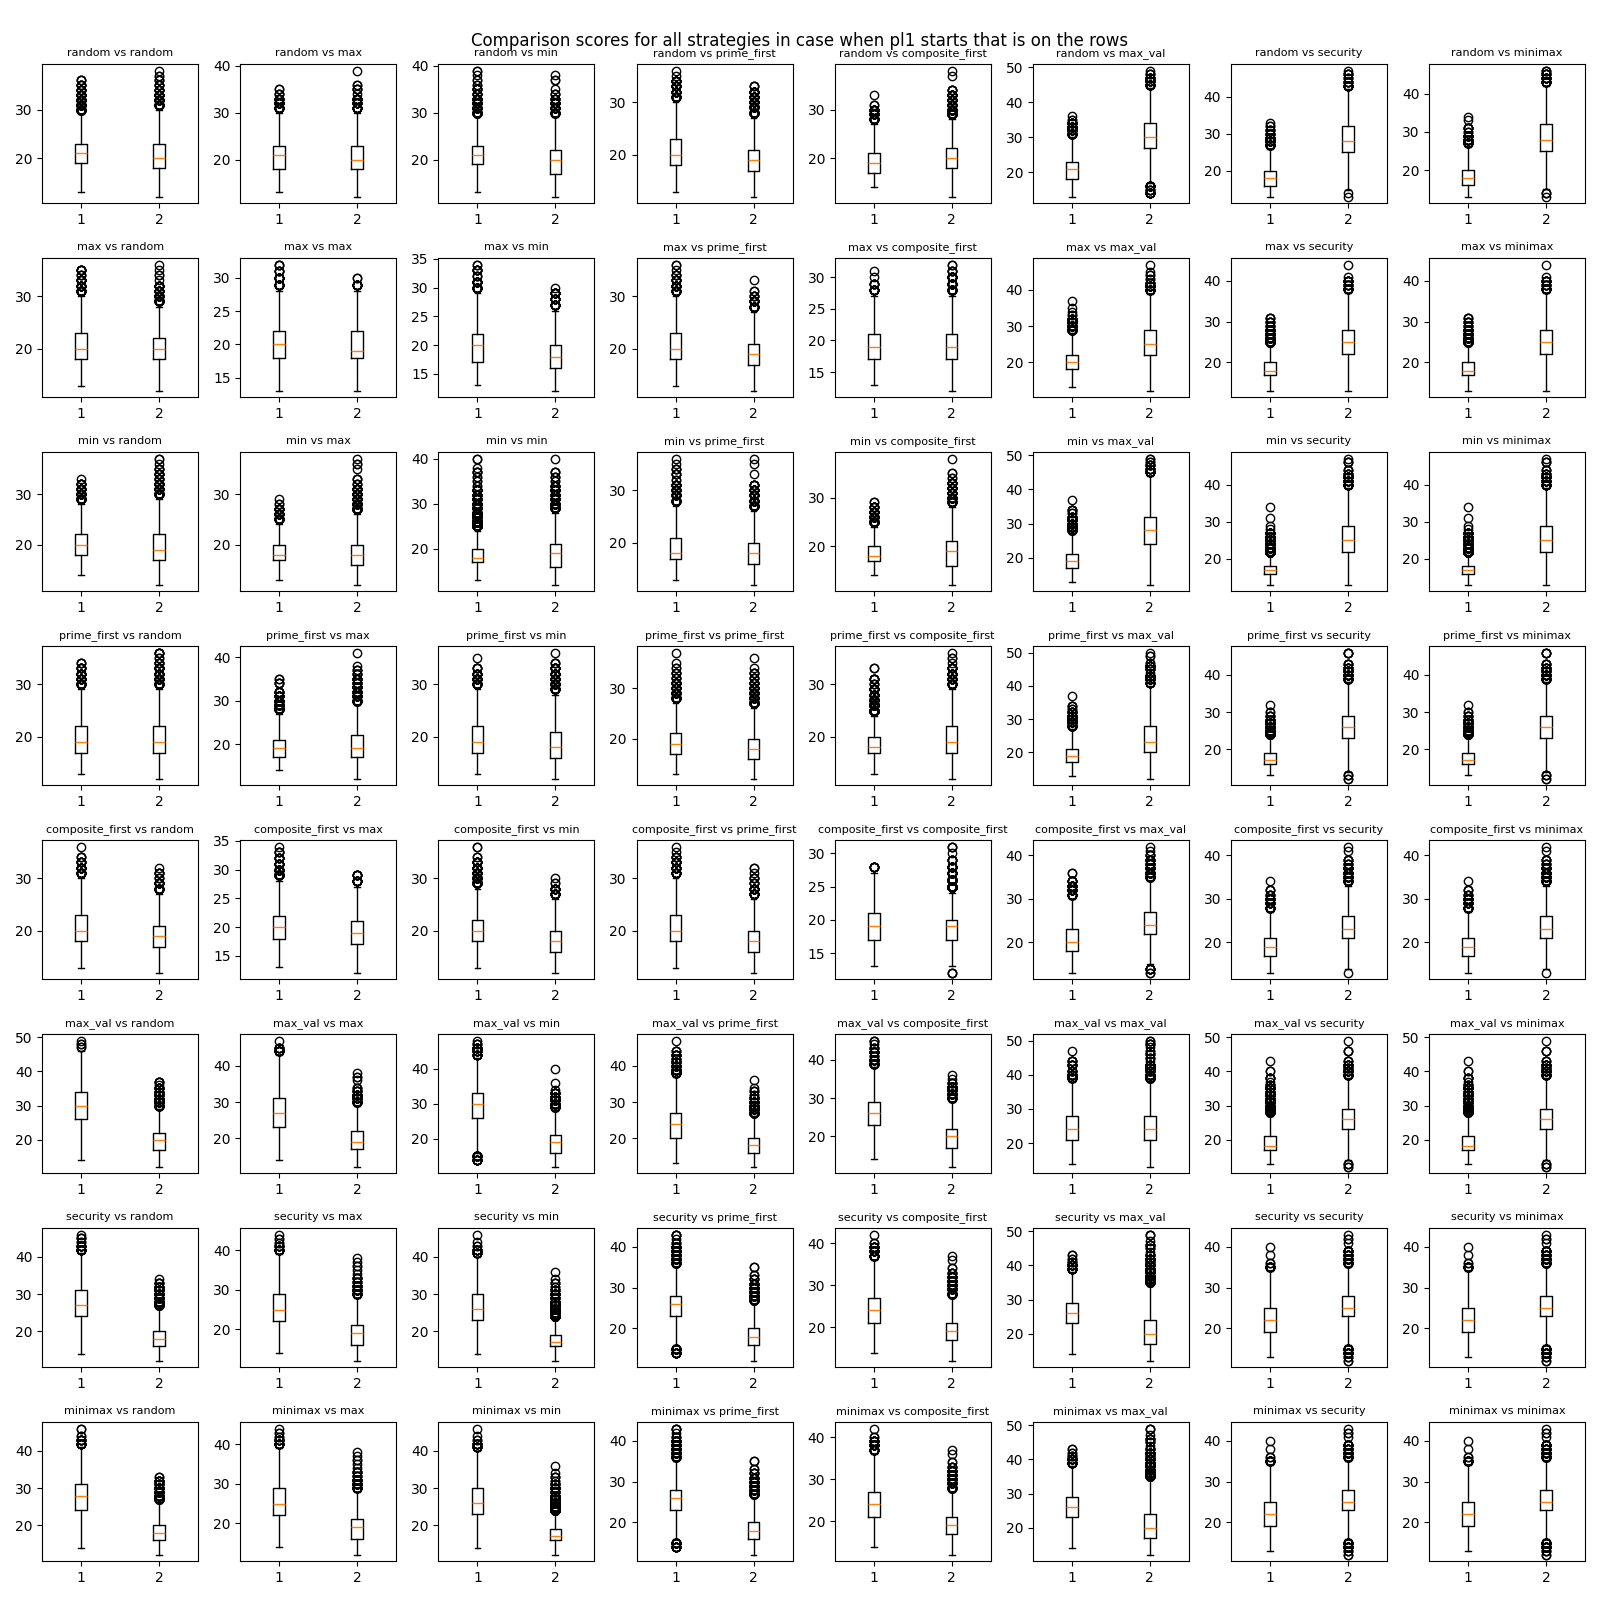
\includegraphics[width=1\linewidth]{img/scores_p1first.png}
	\caption{Plot that reports the box plots of the different score for each pair of strategies when player 1 starts.}
	\label{fig:box_starts}
\end{figure}

In order to better visualize the distribution of the box plots, we restricted the strategies to random, max\_val, security and minimax, since they are the most significant. The results can be seen in Figures \ref{fig:box_general_rel} and \ref{fig:box_starts_rel}.

\begin{figure}
	\centering
	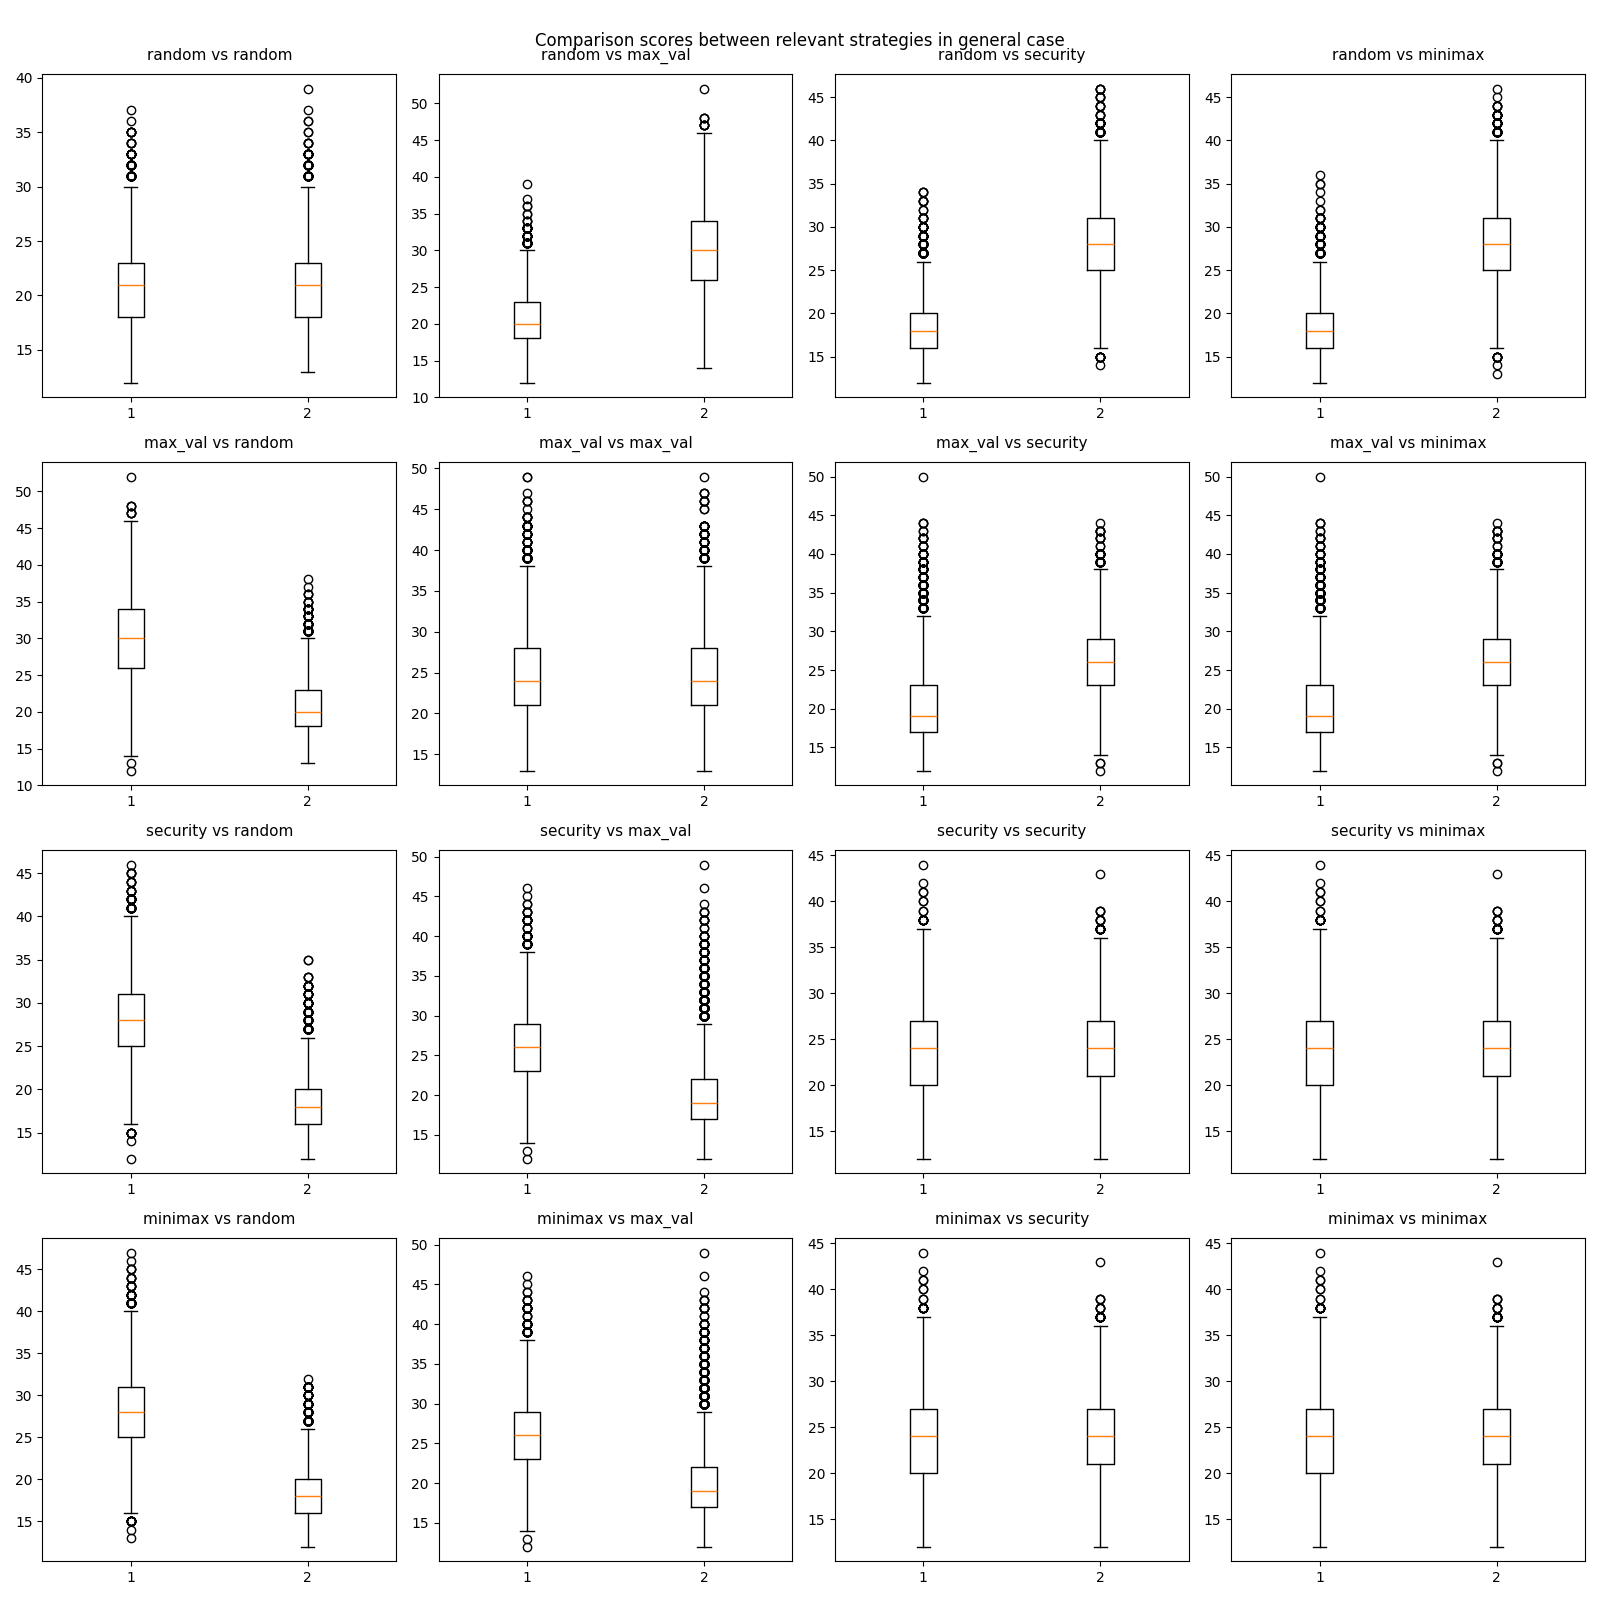
\includegraphics[width=1\linewidth]{img/scores_general_rel.png}
	\caption{Plot that reports the box plots of the different score for each pair of strategies in the general case.}
	\label{fig:box_general_rel}
\end{figure}

\begin{figure}
	\centering
	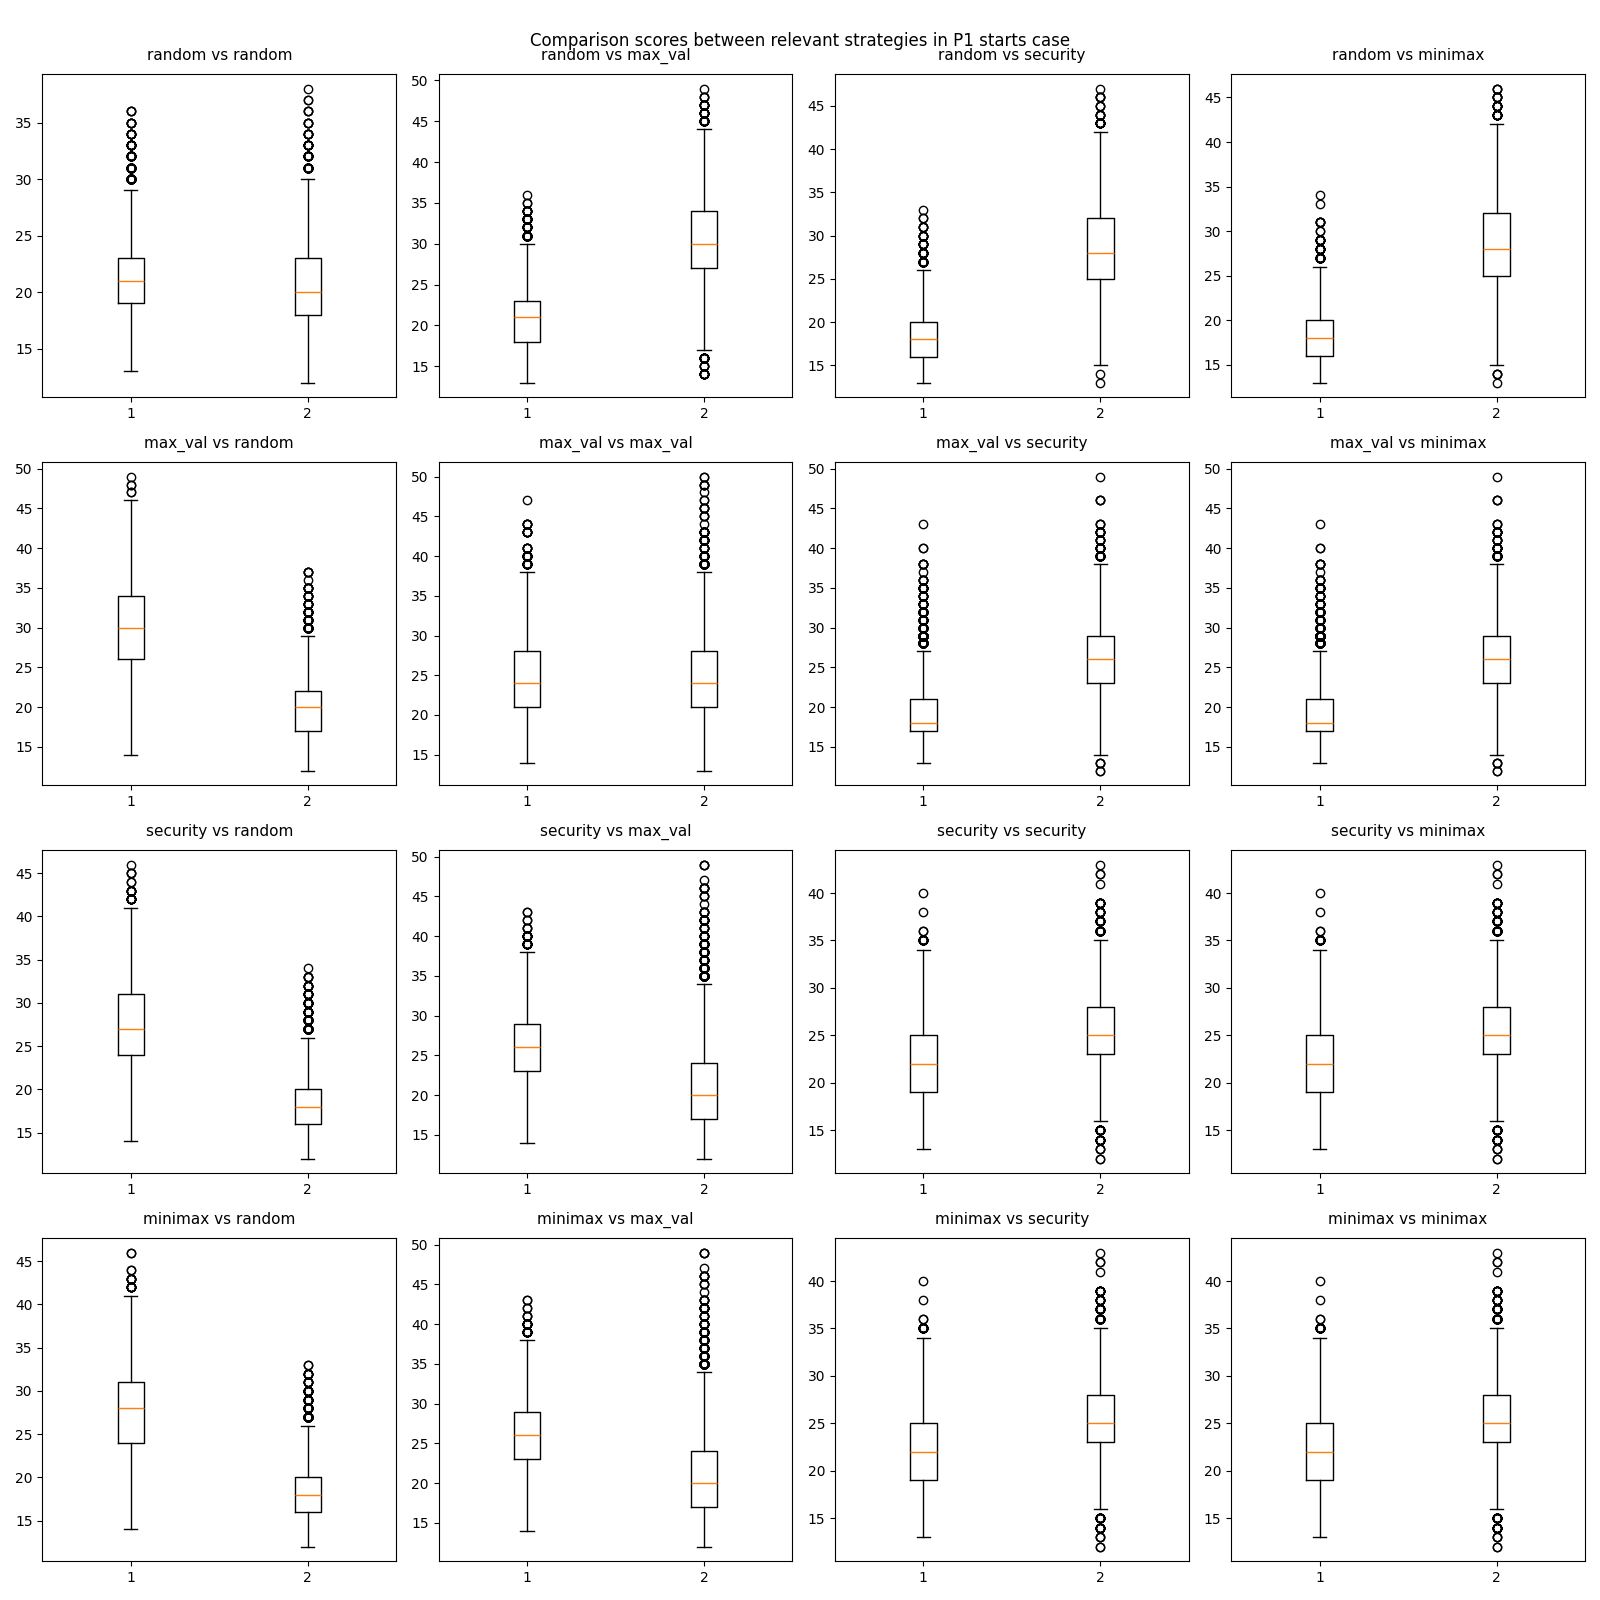
\includegraphics[width=1\linewidth]{img/scores_p1first_rel.png}
	\caption{Plot that reports the box plots of the different score for each pair of strategies when player 1 starts.}
	\label{fig:box_starts_rel}
\end{figure}

From the comparison between those restricted plots, we can see again reflected many of the results discussed in Section \ref{subsection: Outcomes}.
We can see again the bottom left part where we have a worsening of the scores of player 1 from general to the case where it starts confirming again what we have said before. 
Also, we can see that, in general, we have very small boxes but very large whiskers; this means that we have a large variance of the scores but also that in the 2\textsuperscript{nd} and 3\textsuperscript{rd} quantiles we have data that is very concentrated. We can also see that there are a lot of outliers pretty much everywhere. In particular, we can see that when player 1 starts, the number of outliers increases a lot for both players.

At the end of the code, there is also a small part that uses an optimization method to find the binomial distribution that best fits the data in the two cases. The distributions found are very similar to the ones computed before.
